\documentclass[twoside]{book}

% Packages required by doxygen
\usepackage{fixltx2e}
\usepackage{calc}
\usepackage{doxygen}
\usepackage[export]{adjustbox} % also loads graphicx
\usepackage{graphicx}
\usepackage[utf8]{inputenc}
\usepackage{makeidx}
\usepackage{multicol}
\usepackage{multirow}
\PassOptionsToPackage{warn}{textcomp}
\usepackage{textcomp}
\usepackage[nointegrals]{wasysym}
\usepackage[table]{xcolor}

% NLS support packages
\usepackage{polski}
\usepackage[T1]{fontenc}

% Font selection
\usepackage[T1]{fontenc}
\usepackage[scaled=.90]{helvet}
\usepackage{courier}
\usepackage{amssymb}
\usepackage{sectsty}
\renewcommand{\familydefault}{\sfdefault}
\allsectionsfont{%
  \fontseries{bc}\selectfont%
  \color{darkgray}%
}
\renewcommand{\DoxyLabelFont}{%
  \fontseries{bc}\selectfont%
  \color{darkgray}%
}
\newcommand{\+}{\discretionary{\mbox{\scriptsize$\hookleftarrow$}}{}{}}

% Page & text layout
\usepackage{geometry}
\geometry{%
  a4paper,%
  top=2.5cm,%
  bottom=2.5cm,%
  left=2.5cm,%
  right=2.5cm%
}
\tolerance=750
\hfuzz=15pt
\hbadness=750
\setlength{\emergencystretch}{15pt}
\setlength{\parindent}{0cm}
\setlength{\parskip}{3ex plus 2ex minus 2ex}
\makeatletter
\renewcommand{\paragraph}{%
  \@startsection{paragraph}{4}{0ex}{-1.0ex}{1.0ex}{%
    \normalfont\normalsize\bfseries\SS@parafont%
  }%
}
\renewcommand{\subparagraph}{%
  \@startsection{subparagraph}{5}{0ex}{-1.0ex}{1.0ex}{%
    \normalfont\normalsize\bfseries\SS@subparafont%
  }%
}
\makeatother

% Headers & footers
\usepackage{fancyhdr}
\pagestyle{fancyplain}
\fancyhead[LE]{\fancyplain{}{\bfseries\thepage}}
\fancyhead[CE]{\fancyplain{}{}}
\fancyhead[RE]{\fancyplain{}{\bfseries\leftmark}}
\fancyhead[LO]{\fancyplain{}{\bfseries\rightmark}}
\fancyhead[CO]{\fancyplain{}{}}
\fancyhead[RO]{\fancyplain{}{\bfseries\thepage}}
\fancyfoot[LE]{\fancyplain{}{}}
\fancyfoot[CE]{\fancyplain{}{}}
\fancyfoot[RE]{\fancyplain{}{\bfseries\scriptsize Wygenerowano przez Doxygen }}
\fancyfoot[LO]{\fancyplain{}{\bfseries\scriptsize Wygenerowano przez Doxygen }}
\fancyfoot[CO]{\fancyplain{}{}}
\fancyfoot[RO]{\fancyplain{}{}}
\renewcommand{\footrulewidth}{0.4pt}
\renewcommand{\chaptermark}[1]{%
  \markboth{#1}{}%
}
\renewcommand{\sectionmark}[1]{%
  \markright{\thesection\ #1}%
}

% Indices & bibliography
\usepackage{natbib}
\usepackage[titles]{tocloft}
\setcounter{tocdepth}{3}
\setcounter{secnumdepth}{5}
\makeindex

% Hyperlinks (required, but should be loaded last)
\usepackage{ifpdf}
\ifpdf
  \usepackage[pdftex,pagebackref=true]{hyperref}
\else
  \usepackage[ps2pdf,pagebackref=true]{hyperref}
\fi
\hypersetup{%
  colorlinks=true,%
  linkcolor=blue,%
  citecolor=blue,%
  unicode%
}

% Custom commands
\newcommand{\clearemptydoublepage}{%
  \newpage{\pagestyle{empty}\cleardoublepage}%
}

\usepackage{caption}
\captionsetup{labelsep=space,justification=centering,font={bf},singlelinecheck=off,skip=4pt,position=top}

%===== C O N T E N T S =====

\begin{document}

% Titlepage & ToC
\hypersetup{pageanchor=false,
             bookmarksnumbered=true,
             pdfencoding=unicode
            }
\pagenumbering{alph}
\begin{titlepage}
\vspace*{7cm}
\begin{center}%
{\Large Wyszukiwanie cyklów w grafie }\\
\vspace*{1cm}
{\large Wygenerowano przez Doxygen 1.8.13}\\
\end{center}
\end{titlepage}
\clearemptydoublepage
\pagenumbering{roman}
\tableofcontents
\clearemptydoublepage
\pagenumbering{arabic}
\hypersetup{pageanchor=true}

%--- Begin generated contents ---
\chapter{Indeks klas}
\section{Lista klas}
Tutaj znajdują się klasy, struktury, unie i interfejsy wraz z ich krótkimi opisami\+:\begin{DoxyCompactList}
\item\contentsline{section}{\hyperlink{structojciec}{ojciec} }{\pageref{structojciec}}{}
\item\contentsline{section}{\hyperlink{structwierzcholek}{wierzcholek} }{\pageref{structwierzcholek}}{}
\end{DoxyCompactList}

\chapter{Indeks plików}
\section{Lista plików}
Tutaj znajduje się lista wszystkich udokumentowanych plików z ich krótkimi opisami\+:\begin{DoxyCompactList}
\item\contentsline{section}{\hyperlink{funkcje_8cpp}{funkcje.\+cpp} }{\pageref{funkcje_8cpp}}{}
\item\contentsline{section}{{\bfseries funkcje.\+h} }{\pageref{funkcje_8h}}{}
\item\contentsline{section}{\hyperlink{main_8cpp}{main.\+cpp} }{\pageref{main_8cpp}}{}
\item\contentsline{section}{{\bfseries struktury.\+h} }{\pageref{struktury_8h}}{}
\end{DoxyCompactList}

\chapter{Dokumentacja klas}
\hypertarget{structojciec}{}\section{Dokumentacja struktury ojciec}
\label{structojciec}\index{ojciec@{ojciec}}


{\ttfamily \#include $<$struktury.\+h$>$}



Diagram współpracy dla ojciec\+:\nopagebreak
\begin{figure}[H]
\begin{center}
\leavevmode
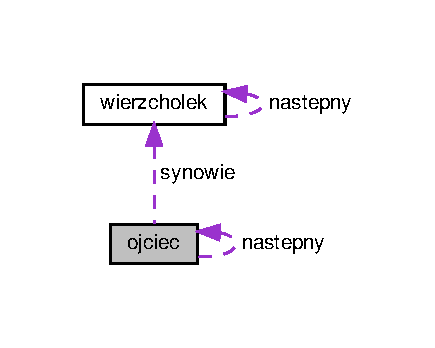
\includegraphics[width=209pt]{structojciec__coll__graph}
\end{center}
\end{figure}
\subsection*{Atrybuty publiczne}
\begin{DoxyCompactItemize}
\item 
int \hyperlink{structojciec_a00cd793091881a3fe5244e47248c674e}{dane}
\item 
bool \hyperlink{structojciec_ab6946ed8062440756408c1608c9614da}{odwiedzony}
\item 
\hyperlink{structwierzcholek}{wierzcholek} $\ast$ \hyperlink{structojciec_a73c0e6fc33374aea30d4b54a0a636d04}{synowie}
\item 
\hyperlink{structojciec}{ojciec} $\ast$ \hyperlink{structojciec_a80e11ec3ccb56da59f2145a171e8e436}{nastepny}
\end{DoxyCompactItemize}


\subsection{Opis szczegółowy}
Struktura reprezentująca graf. Jest to lista list wierzchołków (synów) wychodzących z danego ojca 

\subsection{Dokumentacja atrybutów składowych}
\mbox{\Hypertarget{structojciec_a00cd793091881a3fe5244e47248c674e}\label{structojciec_a00cd793091881a3fe5244e47248c674e}} 
\index{ojciec@{ojciec}!dane@{dane}}
\index{dane@{dane}!ojciec@{ojciec}}
\subsubsection{\texorpdfstring{dane}{dane}}
{\footnotesize\ttfamily int ojciec\+::dane}

wierzchołek \mbox{\Hypertarget{structojciec_a80e11ec3ccb56da59f2145a171e8e436}\label{structojciec_a80e11ec3ccb56da59f2145a171e8e436}} 
\index{ojciec@{ojciec}!nastepny@{nastepny}}
\index{nastepny@{nastepny}!ojciec@{ojciec}}
\subsubsection{\texorpdfstring{nastepny}{nastepny}}
{\footnotesize\ttfamily \hyperlink{structojciec}{ojciec}$\ast$ ojciec\+::nastepny}

wskaźnik na następnego ojca \mbox{\Hypertarget{structojciec_ab6946ed8062440756408c1608c9614da}\label{structojciec_ab6946ed8062440756408c1608c9614da}} 
\index{ojciec@{ojciec}!odwiedzony@{odwiedzony}}
\index{odwiedzony@{odwiedzony}!ojciec@{ojciec}}
\subsubsection{\texorpdfstring{odwiedzony}{odwiedzony}}
{\footnotesize\ttfamily bool ojciec\+::odwiedzony}

czy został odwiedzony \mbox{\Hypertarget{structojciec_a73c0e6fc33374aea30d4b54a0a636d04}\label{structojciec_a73c0e6fc33374aea30d4b54a0a636d04}} 
\index{ojciec@{ojciec}!synowie@{synowie}}
\index{synowie@{synowie}!ojciec@{ojciec}}
\subsubsection{\texorpdfstring{synowie}{synowie}}
{\footnotesize\ttfamily \hyperlink{structwierzcholek}{wierzcholek}$\ast$ ojciec\+::synowie}

wskaźnik na listę synów 

Dokumentacja dla tej struktury została wygenerowana z pliku\+:\begin{DoxyCompactItemize}
\item 
struktury.\+h\end{DoxyCompactItemize}

\hypertarget{structwierzcholek}{}\section{Dokumentacja struktury wierzcholek}
\label{structwierzcholek}\index{wierzcholek@{wierzcholek}}


{\ttfamily \#include $<$struktury.\+h$>$}



Diagram współpracy dla wierzcholek\+:\nopagebreak
\begin{figure}[H]
\begin{center}
\leavevmode

\includegraphics[width=209pt]{structwierzcholek__coll__graph}
\end{center}
\end{figure}
\subsection*{Atrybuty publiczne}
\begin{DoxyCompactItemize}
\item 
int \hyperlink{structwierzcholek_a05773e7b31c7c25b3458a990ec92eb5c}{dane}
\item 
\hyperlink{structwierzcholek}{wierzcholek} $\ast$ \hyperlink{structwierzcholek_afc6e289ba34df6780a3b73f8f189a878}{nastepny}
\end{DoxyCompactItemize}


\subsection{Opis szczegółowy}
Lista trzymająca kolejne wierzchołki wychodzące ze wspólnego ojca. 

\subsection{Dokumentacja atrybutów składowych}
\mbox{\Hypertarget{structwierzcholek_a05773e7b31c7c25b3458a990ec92eb5c}\label{structwierzcholek_a05773e7b31c7c25b3458a990ec92eb5c}} 
\index{wierzcholek@{wierzcholek}!dane@{dane}}
\index{dane@{dane}!wierzcholek@{wierzcholek}}
\subsubsection{\texorpdfstring{dane}{dane}}
{\footnotesize\ttfamily int wierzcholek\+::dane}

wierzchołek \mbox{\Hypertarget{structwierzcholek_afc6e289ba34df6780a3b73f8f189a878}\label{structwierzcholek_afc6e289ba34df6780a3b73f8f189a878}} 
\index{wierzcholek@{wierzcholek}!nastepny@{nastepny}}
\index{nastepny@{nastepny}!wierzcholek@{wierzcholek}}
\subsubsection{\texorpdfstring{nastepny}{nastepny}}
{\footnotesize\ttfamily \hyperlink{structwierzcholek}{wierzcholek}$\ast$ wierzcholek\+::nastepny}

wskaźnik do następnego wierzchołka 

Dokumentacja dla tej struktury została wygenerowana z pliku\+:\begin{DoxyCompactItemize}
\item 
struktury.\+h\end{DoxyCompactItemize}

\chapter{Dokumentacja plików}
\hypertarget{funkcje_8cpp}{}\section{Dokumentacja pliku funkcje.\+cpp}
\label{funkcje_8cpp}\index{funkcje.\+cpp@{funkcje.\+cpp}}
{\ttfamily \#include $<$iostream$>$}\newline
{\ttfamily \#include $<$string$>$}\newline
{\ttfamily \#include $<$iomanip$>$}\newline
{\ttfamily \#include $<$cmath$>$}\newline
{\ttfamily \#include $<$cstdio$>$}\newline
{\ttfamily \#include $<$cstdlib$>$}\newline
{\ttfamily \#include $<$fstream$>$}\newline
{\ttfamily \#include \char`\"{}funkcje.\+h\char`\"{}}\newline
Wykres zależności załączania dla funkcje.\+cpp\+:\nopagebreak
\begin{figure}[H]
\begin{center}
\leavevmode
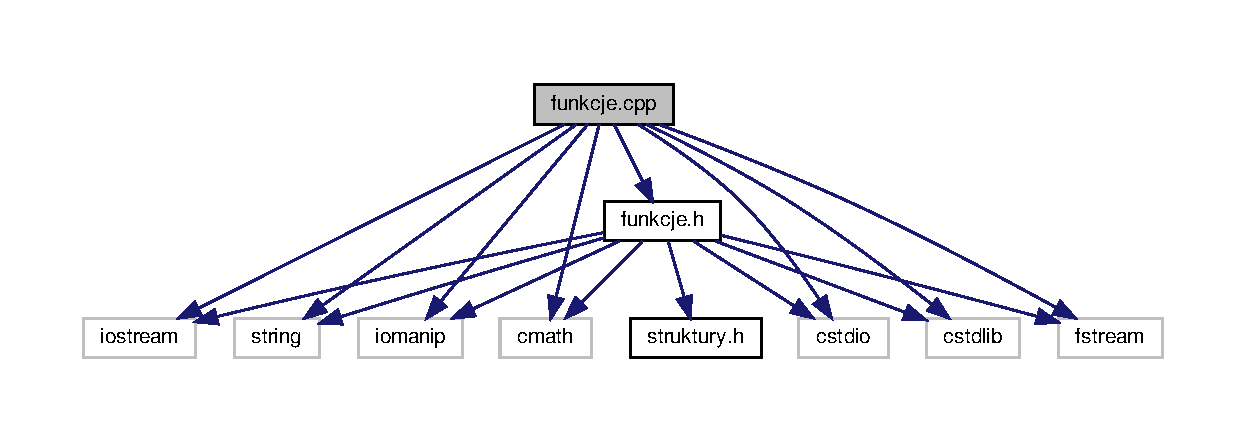
\includegraphics[width=350pt]{funkcje_8cpp__incl}
\end{center}
\end{figure}
\subsection*{Funkcje}
\begin{DoxyCompactItemize}
\item 
\hyperlink{structojciec}{ojciec} $\ast$ \hyperlink{funkcje_8cpp_a745d4c883df53b14a22e4e71cca25512}{wyszukaj\+\_\+ojca} (\hyperlink{structojciec}{ojciec} $\ast$graf\+Head, int ojciec\+\_\+dane)
\item 
void \hyperlink{funkcje_8cpp_ae4530c49bef00f8c7ecb6cd88ebfee15}{dodaj\+\_\+ojca} (\hyperlink{structojciec}{ojciec} $\ast$\&graf\+Head, int ojciec\+\_\+dane)
\item 
void \hyperlink{funkcje_8cpp_a397d5f5b870965200cb1733450ac8070}{dodaj\+\_\+syna} (\hyperlink{structojciec}{ojciec} $\ast$\&ojciec\+Syna, int syn\+Dane)
\item 
void \hyperlink{funkcje_8cpp_aed4262ab3b2f96fed3e0d86997e1f7c0}{dodaj\+\_\+dane} (int ojciec\+Dane, int syn\+Dane, \hyperlink{structojciec}{ojciec} $\ast$\&graf\+Head)
\item 
void \hyperlink{funkcje_8cpp_a1983566de3ac83afb818a74158ab200d}{wczytaj\+\_\+graf} (std\+::string plik, \hyperlink{structojciec}{ojciec} $\ast$\&start\+\_\+grafu)
\item 
void \hyperlink{funkcje_8cpp_aafb80c1ac88f78656e5d654488ca8417}{wypisz\+\_\+graf} (\hyperlink{structojciec}{ojciec} $\ast$graf\+Head)
\item 
void \hyperlink{funkcje_8cpp_adf963e4d7b897a21f81d49c21880322c}{dodaj\+\_\+do\+\_\+listy} (\hyperlink{structojciec}{ojciec} $\ast$\&lista\+Head, \hyperlink{structwierzcholek}{wierzcholek} $\ast$\&cykl, int iterator)
\item 
\mbox{\Hypertarget{funkcje_8cpp_a1230a763f975e41e41c0bd0b97d6349f}\label{funkcje_8cpp_a1230a763f975e41e41c0bd0b97d6349f}} 
void {\bfseries wypisz\+\_\+stos\+\_\+od\+\_\+tylu} (\hyperlink{structwierzcholek}{wierzcholek} $\ast$stos, std\+::ofstream $\ast$plik\+Wy)
\item 
\mbox{\Hypertarget{funkcje_8cpp_a7fb49a548f1f7d0d65dd0dc5e611fb20}\label{funkcje_8cpp_a7fb49a548f1f7d0d65dd0dc5e611fb20}} 
void {\bfseries dodaj\+\_\+do\+\_\+stosu} (\hyperlink{structwierzcholek}{wierzcholek} $\ast$\&stos, int wartosc)
\item 
\mbox{\Hypertarget{funkcje_8cpp_a208ab2fb28b91f723aba4c2c7952ad30}\label{funkcje_8cpp_a208ab2fb28b91f723aba4c2c7952ad30}} 
void {\bfseries zdejmij\+\_\+ze\+\_\+stosu} (\hyperlink{structwierzcholek}{wierzcholek} $\ast$\&stos)
\item 
void \hyperlink{funkcje_8cpp_a8e4b7b83059f72ecea2dcffe4d38500a}{D\+FS} (\hyperlink{structojciec}{ojciec} $\ast$\&graf\+Head, int poczatek, \hyperlink{structwierzcholek}{wierzcholek} $\ast$\&lista, int pierwszy, std\+::ofstream $\ast$plik\+Wy, int \&counter)
\item 
void \hyperlink{funkcje_8cpp_a0841ba57b8bbd7ad54567a89ace1fefe}{wyczysc\+\_\+odwiedzone} (\hyperlink{structojciec}{ojciec} $\ast$\&graf\+Head)
\item 
void \hyperlink{funkcje_8cpp_ad840d380915ccca02b7f859f626d86a0}{usun} (\hyperlink{structojciec}{ojciec} $\ast$\&graf\+Head)
\item 
void \hyperlink{funkcje_8cpp_a56885cc99ce389819da209443e3d0ef8}{usun} (\hyperlink{structwierzcholek}{wierzcholek} $\ast$\&graf\+Head)
\end{DoxyCompactItemize}


\subsection{Dokumentacja funkcji}
\mbox{\Hypertarget{funkcje_8cpp_a8e4b7b83059f72ecea2dcffe4d38500a}\label{funkcje_8cpp_a8e4b7b83059f72ecea2dcffe4d38500a}} 
\index{funkcje.\+cpp@{funkcje.\+cpp}!D\+FS@{D\+FS}}
\index{D\+FS@{D\+FS}!funkcje.\+cpp@{funkcje.\+cpp}}
\subsubsection{\texorpdfstring{D\+F\+S()}{DFS()}}
{\footnotesize\ttfamily void D\+FS (\begin{DoxyParamCaption}\item[{\hyperlink{structojciec}{ojciec} $\ast$\&}]{graf\+Head,  }\item[{int}]{poczatek,  }\item[{\hyperlink{structwierzcholek}{wierzcholek} $\ast$\&}]{lista,  }\item[{int}]{pierwszy,  }\item[{std\+::ofstream $\ast$}]{plik\+Wy,  }\item[{int \&}]{counter }\end{DoxyParamCaption})}

Funkcja będąca implementacją algorytmu D\+FS na listach podwieszanych 
\begin{DoxyParams}{Parametry}
{\em graf\+Head} & graf, którym przechodzimy \\
\hline
{\em poczatek} & początkowy wierzchołek do przechodzenia grafu \\
\hline
{\em lista} & pomocnicza lista do trzymania stosu wierzchołków \\
\hline
{\em pierwszy} & początkowy wierzchołek, do którego ścieżki szukamy \\
\hline
{\em plik\+Wy} & plik wyjściowy \\
\hline
{\em counter} & licznik cykli \\
\hline
\end{DoxyParams}
\mbox{\Hypertarget{funkcje_8cpp_aed4262ab3b2f96fed3e0d86997e1f7c0}\label{funkcje_8cpp_aed4262ab3b2f96fed3e0d86997e1f7c0}} 
\index{funkcje.\+cpp@{funkcje.\+cpp}!dodaj\+\_\+dane@{dodaj\+\_\+dane}}
\index{dodaj\+\_\+dane@{dodaj\+\_\+dane}!funkcje.\+cpp@{funkcje.\+cpp}}
\subsubsection{\texorpdfstring{dodaj\+\_\+dane()}{dodaj\_dane()}}
{\footnotesize\ttfamily void dodaj\+\_\+dane (\begin{DoxyParamCaption}\item[{int}]{ojciec\+Dane,  }\item[{int}]{syn\+Dane,  }\item[{\hyperlink{structojciec}{ojciec} $\ast$\&}]{graf\+Head }\end{DoxyParamCaption})}

Funkcja dodająca syna do listy ojca 
\begin{DoxyParams}{Parametry}
{\em ojciec\+Dane} & wartość ojca \\
\hline
{\em syn\+Dane} & wartość syna \\
\hline
{\em graf\+Head} & adres grafu \\
\hline
\end{DoxyParams}
\mbox{\Hypertarget{funkcje_8cpp_adf963e4d7b897a21f81d49c21880322c}\label{funkcje_8cpp_adf963e4d7b897a21f81d49c21880322c}} 
\index{funkcje.\+cpp@{funkcje.\+cpp}!dodaj\+\_\+do\+\_\+listy@{dodaj\+\_\+do\+\_\+listy}}
\index{dodaj\+\_\+do\+\_\+listy@{dodaj\+\_\+do\+\_\+listy}!funkcje.\+cpp@{funkcje.\+cpp}}
\subsubsection{\texorpdfstring{dodaj\+\_\+do\+\_\+listy()}{dodaj\_do\_listy()}}
{\footnotesize\ttfamily void dodaj\+\_\+do\+\_\+listy (\begin{DoxyParamCaption}\item[{\hyperlink{structojciec}{ojciec} $\ast$\&}]{lista\+Head,  }\item[{\hyperlink{structwierzcholek}{wierzcholek} $\ast$\&}]{cykl,  }\item[{int}]{iterator }\end{DoxyParamCaption})}

Funkcja dodająca listę z cyklem do listy głównej, zawierającej wszystkie cykle 
\begin{DoxyParams}{Parametry}
{\em list\+Head} & lista, do której dodajemy cykle \\
\hline
\end{DoxyParams}
\mbox{\Hypertarget{funkcje_8cpp_ae4530c49bef00f8c7ecb6cd88ebfee15}\label{funkcje_8cpp_ae4530c49bef00f8c7ecb6cd88ebfee15}} 
\index{funkcje.\+cpp@{funkcje.\+cpp}!dodaj\+\_\+ojca@{dodaj\+\_\+ojca}}
\index{dodaj\+\_\+ojca@{dodaj\+\_\+ojca}!funkcje.\+cpp@{funkcje.\+cpp}}
\subsubsection{\texorpdfstring{dodaj\+\_\+ojca()}{dodaj\_ojca()}}
{\footnotesize\ttfamily void dodaj\+\_\+ojca (\begin{DoxyParamCaption}\item[{\hyperlink{structojciec}{ojciec} $\ast$\&}]{graf\+Head,  }\item[{int}]{ojciec\+Dane }\end{DoxyParamCaption})}

Funkcja dodająca ojca do grafu 
\begin{DoxyParams}{Parametry}
{\em graf\+Head} & graf, w którym dodajemy ojca \\
\hline
{\em ojciec\+Dane} & wartość ojca, którą dodajemy do grafu \\
\hline
\end{DoxyParams}
\mbox{\Hypertarget{funkcje_8cpp_a397d5f5b870965200cb1733450ac8070}\label{funkcje_8cpp_a397d5f5b870965200cb1733450ac8070}} 
\index{funkcje.\+cpp@{funkcje.\+cpp}!dodaj\+\_\+syna@{dodaj\+\_\+syna}}
\index{dodaj\+\_\+syna@{dodaj\+\_\+syna}!funkcje.\+cpp@{funkcje.\+cpp}}
\subsubsection{\texorpdfstring{dodaj\+\_\+syna()}{dodaj\_syna()}}
{\footnotesize\ttfamily void dodaj\+\_\+syna (\begin{DoxyParamCaption}\item[{\hyperlink{structojciec}{ojciec} $\ast$\&}]{ojciec\+Syna,  }\item[{int}]{syn\+Dane }\end{DoxyParamCaption})}

Funkcja dodająca syna do list adjacencji ojca 
\begin{DoxyParams}{Parametry}
{\em ojciec\+Syna} & adres ojca, do listy którego dodajemy syna \\
\hline
{\em syn\+Dane} & wartość syna, którego dodajemy do list ojca \\
\hline
\end{DoxyParams}
\mbox{\Hypertarget{funkcje_8cpp_ad840d380915ccca02b7f859f626d86a0}\label{funkcje_8cpp_ad840d380915ccca02b7f859f626d86a0}} 
\index{funkcje.\+cpp@{funkcje.\+cpp}!usun@{usun}}
\index{usun@{usun}!funkcje.\+cpp@{funkcje.\+cpp}}
\subsubsection{\texorpdfstring{usun()}{usun()}\hspace{0.1cm}{\footnotesize\ttfamily [1/2]}}
{\footnotesize\ttfamily void usun (\begin{DoxyParamCaption}\item[{\hyperlink{structojciec}{ojciec} $\ast$\&}]{graf\+Head }\end{DoxyParamCaption})}

Funkcja usuwająca graf 
\begin{DoxyParams}{Parametry}
{\em graf\+Head} & graf do usunięcia \\
\hline
\end{DoxyParams}
\mbox{\Hypertarget{funkcje_8cpp_a56885cc99ce389819da209443e3d0ef8}\label{funkcje_8cpp_a56885cc99ce389819da209443e3d0ef8}} 
\index{funkcje.\+cpp@{funkcje.\+cpp}!usun@{usun}}
\index{usun@{usun}!funkcje.\+cpp@{funkcje.\+cpp}}
\subsubsection{\texorpdfstring{usun()}{usun()}\hspace{0.1cm}{\footnotesize\ttfamily [2/2]}}
{\footnotesize\ttfamily void usun (\begin{DoxyParamCaption}\item[{\hyperlink{structwierzcholek}{wierzcholek} $\ast$\&}]{graf\+Head }\end{DoxyParamCaption})}

Funkcja usuwająca listę wierzchołków 
\begin{DoxyParams}{Parametry}
{\em graf\+Head} & lista do usunięcia \\
\hline
\end{DoxyParams}
\mbox{\Hypertarget{funkcje_8cpp_a1983566de3ac83afb818a74158ab200d}\label{funkcje_8cpp_a1983566de3ac83afb818a74158ab200d}} 
\index{funkcje.\+cpp@{funkcje.\+cpp}!wczytaj\+\_\+graf@{wczytaj\+\_\+graf}}
\index{wczytaj\+\_\+graf@{wczytaj\+\_\+graf}!funkcje.\+cpp@{funkcje.\+cpp}}
\subsubsection{\texorpdfstring{wczytaj\+\_\+graf()}{wczytaj\_graf()}}
{\footnotesize\ttfamily void wczytaj\+\_\+graf (\begin{DoxyParamCaption}\item[{std\+::string}]{plik,  }\item[{\hyperlink{structojciec}{ojciec} $\ast$\&}]{start\+\_\+grafu }\end{DoxyParamCaption})}

Funkcja wczytująca graf z podanego pliku do pamięci programu. 
\begin{DoxyParams}{Parametry}
{\em plik} & nazwa pliku, z którego należy wczytać graf \\
\hline
{\em graf} & wskaźnik na listę, w której trzymany będzie graf \\
\hline
\end{DoxyParams}
\mbox{\Hypertarget{funkcje_8cpp_a0841ba57b8bbd7ad54567a89ace1fefe}\label{funkcje_8cpp_a0841ba57b8bbd7ad54567a89ace1fefe}} 
\index{funkcje.\+cpp@{funkcje.\+cpp}!wyczysc\+\_\+odwiedzone@{wyczysc\+\_\+odwiedzone}}
\index{wyczysc\+\_\+odwiedzone@{wyczysc\+\_\+odwiedzone}!funkcje.\+cpp@{funkcje.\+cpp}}
\subsubsection{\texorpdfstring{wyczysc\+\_\+odwiedzone()}{wyczysc\_odwiedzone()}}
{\footnotesize\ttfamily void wyczysc\+\_\+odwiedzone (\begin{DoxyParamCaption}\item[{\hyperlink{structojciec}{ojciec} $\ast$\&}]{graf\+Head }\end{DoxyParamCaption})}

Funkcja zerująca znacznik {\ttfamily odwiedzony} w grafie 
\begin{DoxyParams}{Parametry}
{\em graf\+Head} & graf \\
\hline
\end{DoxyParams}
\mbox{\Hypertarget{funkcje_8cpp_aafb80c1ac88f78656e5d654488ca8417}\label{funkcje_8cpp_aafb80c1ac88f78656e5d654488ca8417}} 
\index{funkcje.\+cpp@{funkcje.\+cpp}!wypisz\+\_\+graf@{wypisz\+\_\+graf}}
\index{wypisz\+\_\+graf@{wypisz\+\_\+graf}!funkcje.\+cpp@{funkcje.\+cpp}}
\subsubsection{\texorpdfstring{wypisz\+\_\+graf()}{wypisz\_graf()}}
{\footnotesize\ttfamily void wypisz\+\_\+graf (\begin{DoxyParamCaption}\item[{\hyperlink{structojciec}{ojciec} $\ast$}]{graf\+Head }\end{DoxyParamCaption})}

Funkcja wypisująca tablicę adjacencji (debugging) 
\begin{DoxyParams}{Parametry}
{\em graf\+Head} & graf do wypisania \\
\hline
\end{DoxyParams}
\mbox{\Hypertarget{funkcje_8cpp_a745d4c883df53b14a22e4e71cca25512}\label{funkcje_8cpp_a745d4c883df53b14a22e4e71cca25512}} 
\index{funkcje.\+cpp@{funkcje.\+cpp}!wyszukaj\+\_\+ojca@{wyszukaj\+\_\+ojca}}
\index{wyszukaj\+\_\+ojca@{wyszukaj\+\_\+ojca}!funkcje.\+cpp@{funkcje.\+cpp}}
\subsubsection{\texorpdfstring{wyszukaj\+\_\+ojca()}{wyszukaj\_ojca()}}
{\footnotesize\ttfamily \hyperlink{structojciec}{ojciec}$\ast$ wyszukaj\+\_\+ojca (\begin{DoxyParamCaption}\item[{\hyperlink{structojciec}{ojciec} $\ast$}]{graf\+Head,  }\item[{int}]{ojciec\+Dane }\end{DoxyParamCaption})}

Funkcja wyszukująca adres ojca listy do której należy dodać kolejny wierzchołek. 
\begin{DoxyParams}{Parametry}
{\em graf\+Head} & graf w którym szukamy ojca \\
\hline
{\em ojciec\+Dane} & wartość ojca, którego szukamy \\
\hline
\end{DoxyParams}
\begin{DoxyReturn}{Zwraca}
adres ojca, którego szukano 
\end{DoxyReturn}

\hypertarget{main_8cpp}{}\section{Dokumentacja pliku main.\+cpp}
\label{main_8cpp}\index{main.\+cpp@{main.\+cpp}}
{\ttfamily \#include $<$iostream$>$}\newline
{\ttfamily \#include $<$string$>$}\newline
{\ttfamily \#include $<$iomanip$>$}\newline
{\ttfamily \#include $<$cmath$>$}\newline
{\ttfamily \#include $<$cstdio$>$}\newline
{\ttfamily \#include $<$cstdlib$>$}\newline
{\ttfamily \#include $<$cstring$>$}\newline
{\ttfamily \#include $<$values.\+h$>$}\newline
{\ttfamily \#include $<$fstream$>$}\newline
{\ttfamily \#include \char`\"{}funkcje.\+h\char`\"{}}\newline
{\ttfamily \#include \char`\"{}struktury.\+h\char`\"{}}\newline
Wykres zależności załączania dla main.\+cpp\+:\nopagebreak
\begin{figure}[H]
\begin{center}
\leavevmode
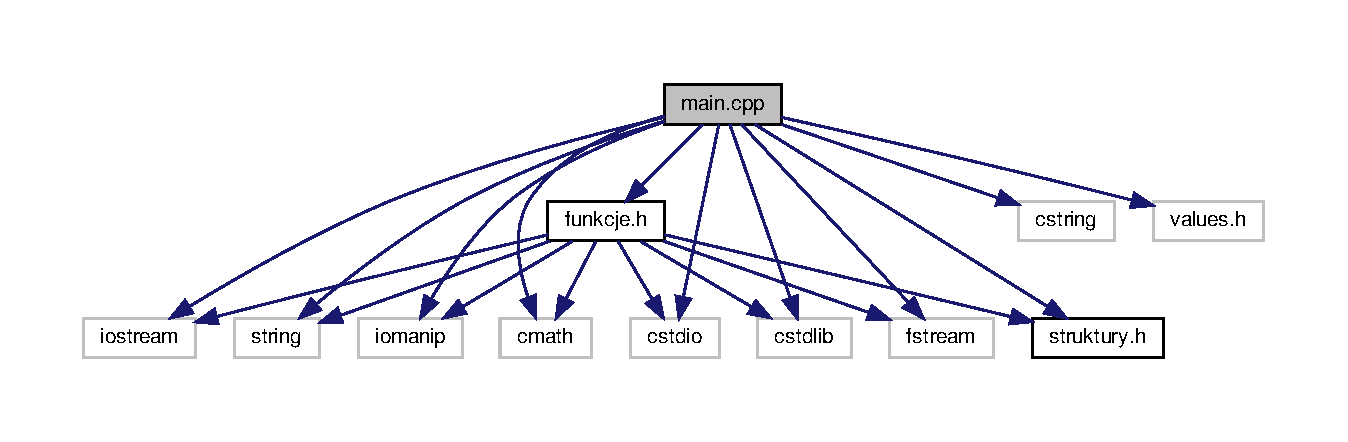
\includegraphics[width=350pt]{main_8cpp__incl}
\end{center}
\end{figure}
\subsection*{Funkcje}
\begin{DoxyCompactItemize}
\item 
\mbox{\Hypertarget{main_8cpp_a0ddf1224851353fc92bfbff6f499fa97}\label{main_8cpp_a0ddf1224851353fc92bfbff6f499fa97}} 
int {\bfseries main} (int argc, char $\ast$argv\mbox{[}$\,$\mbox{]})
\end{DoxyCompactItemize}

%--- End generated contents ---

% Index
\backmatter
\newpage
\phantomsection
\clearemptydoublepage
\addcontentsline{toc}{chapter}{Indeks}
\printindex

\end{document}
